\chapter{Sparse Polynomial Interpolation}
\label{ch:benor-tiwari}

We shall discuss the paper \cite{ben-or-tiwari} here.

\begin{definition}[Sparse Polynomial]
    We call a polynomial $P\in A[x_1,\ldots,x_n]$ \emph{$t$-sparse} if it has at most $t$-many monomials with non-zero coefficient in $P$.
\end{definition}

The main problem of concern for this chapter is the following:

\begin{blackbox}
    \begin{problem}
           How many evaluations are needed to interpolate a $t$-sparse polynomial $P$ deterministically, if we have the $A^n$-evaluation of $P$?
    \end{problem}
\end{blackbox}

\begin{figure}[h]
\centering
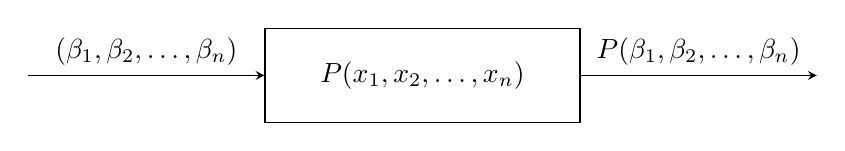
\begin{tikzpicture}[>=stealth]
    \node[draw, rectangle, minimum width=4cm, minimum height=1.2cm, align=center]
        (bb) {$P(x_1, x_2, \ldots, x_n)$};
    \draw[->] ([xshift=-3cm]bb.west) -- (bb.west)
        node[midway, above] {$(\beta_1, \beta_2, \ldots, \beta_n)$};
    \draw[->] (bb.east) -- ([xshift=3cm]bb.east)
        node[midway, above] {$P(\beta_1, \beta_2, \ldots, \beta_n)$};
\end{tikzpicture}
\caption{Black-box model \textup{\cite{ben-or-tiwari}}.}
\label{fig:blackbox}
\end{figure}

